\section{Data Analysis}

\begin{frame}{Data Analysis}{}
	\begin{itemize}
		\item {Simulation Bunches}
		\item {Simulation Handlers}
		\item {Analyzer}
		\item {Empirical Results}
	\end{itemize}
		

\end{frame}

\subsection{Simulation Bunches}	
	\begin{frame}{Simulation Bunches}
		
		\begin{enumerate}
			\item Traced clients fixed to the 100\% and increasing
traced servers at each macro bunch run ($ 0\% \rightarrow 100\% $).
			\item Traced servers fixed to the 100\% and increasing
traced clients at each macro bunch run ($ 0\% \rightarrow 100\% $).
			\item Increainsg both traced clients and traced servers (traced
		 portion) at each simulation ($ 0\% \rightarrow 100\% $).
		\end{enumerate}

	\end{frame}
	\begin{frame}{Simulation Bunches}
		\begin{figure}
			\centering
			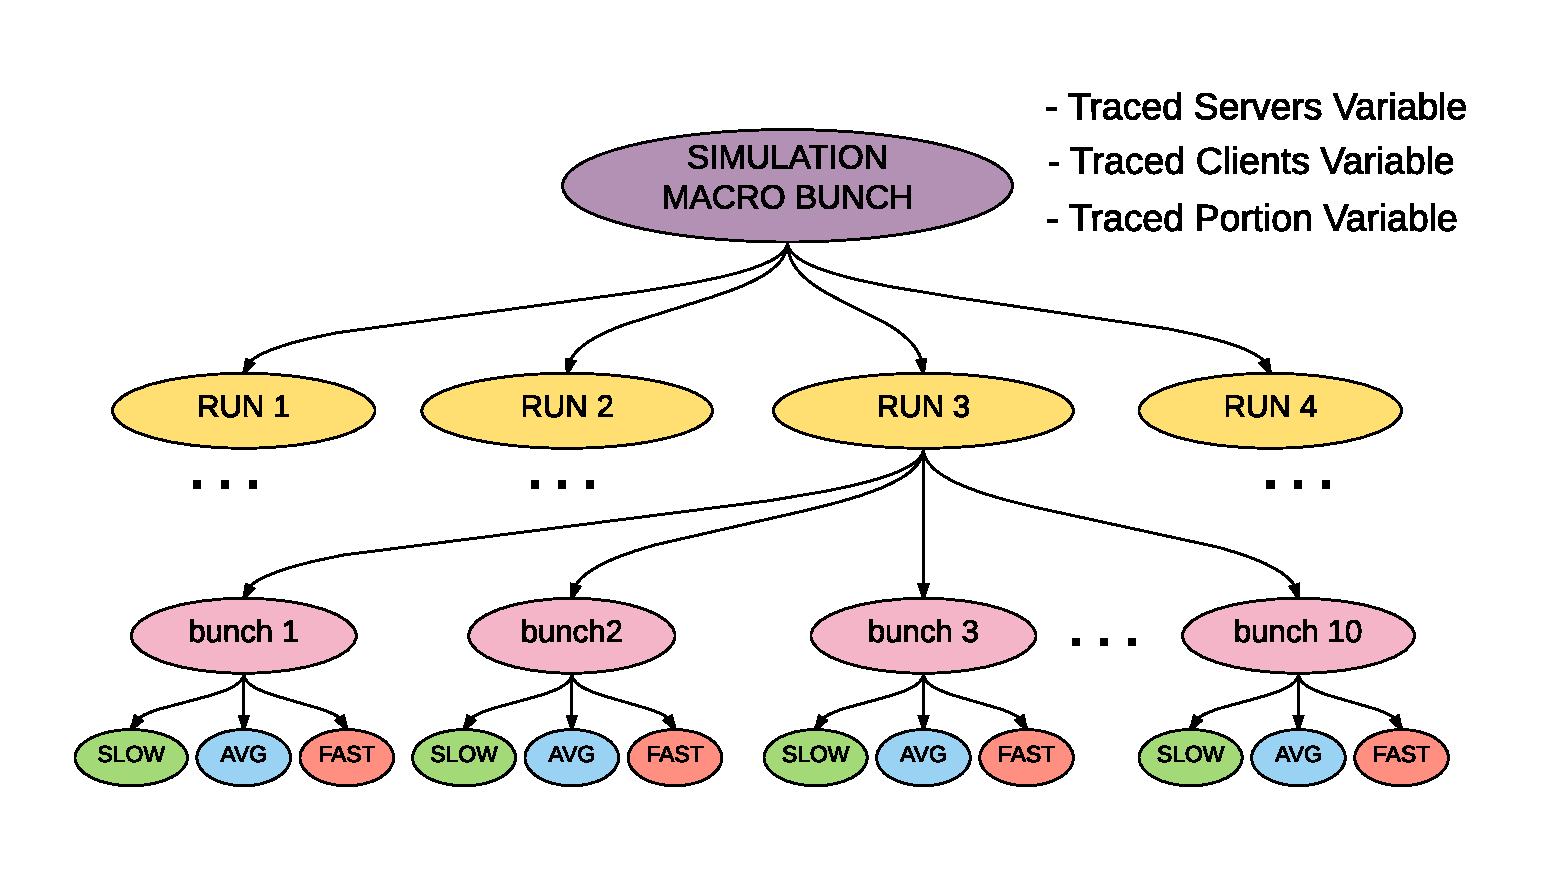
\includegraphics[scale=0.45]{img/bunches.pdf}
		\end{figure}
	\end{frame}	

\subsection{Simulation Handlers}
	\begin{frame}{Simulation Handlers}
		\begin{itemize}
			\item Netbuilder
			\item Launcher
		\end{itemize}
	\end{frame}

	\begin{frame}{Netbuilder}
		Genereates an XML file that describes the network
			
		\begin{figure}
			\centering
			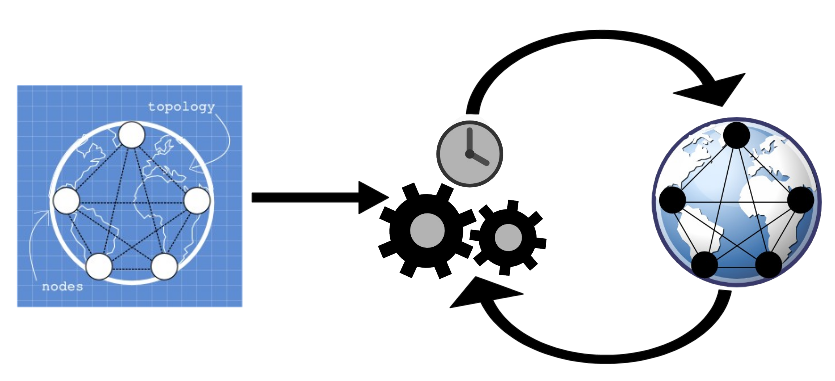
\includegraphics[scale=0.35]{img/design1.png}
		\end{figure}
	\end{frame}

	\begin{frame}{Netbuilder}{Configuration}
		Allow the network configuration through:
		\begin{itemize}
			
			\item The number of TOR exit nodes in the simulation.
			\item The number of TOR 4authorities\footnote{A 4 Authority node is simply the
			database that keep track of the state of the TOR network and the list
			of the TOR relays/exit-nodes} nodes in the simulation.
			\item The number of clients (simpletcp) of the simulation.
			\item The number of servers (simpletcp) of the simulation.
			\item The percentage of clients tracked by an autosys plug-in.
			\item The percentage of servers tracked by an autosys plug-in.
			\item The density of the network-requests.
		\end{itemize}
	\end{frame}	

	\begin{frame}{Netbuilder}{Densities}
		The connection densities are the sleep time thresholds between each client connection request:
			
		\begin{itemize}
			\item Slow: 800 (mean) - 2000 (mean) milliseconds 			
			\item Average: 80 (mean)  - 1000 (mean) millisecons
			\item Fast: 20 (mean) - 100 (mean) milliseconds
		\end{itemize}
	\end{frame}			
	

	\begin{frame}{Launcher}
		\begin{center}
			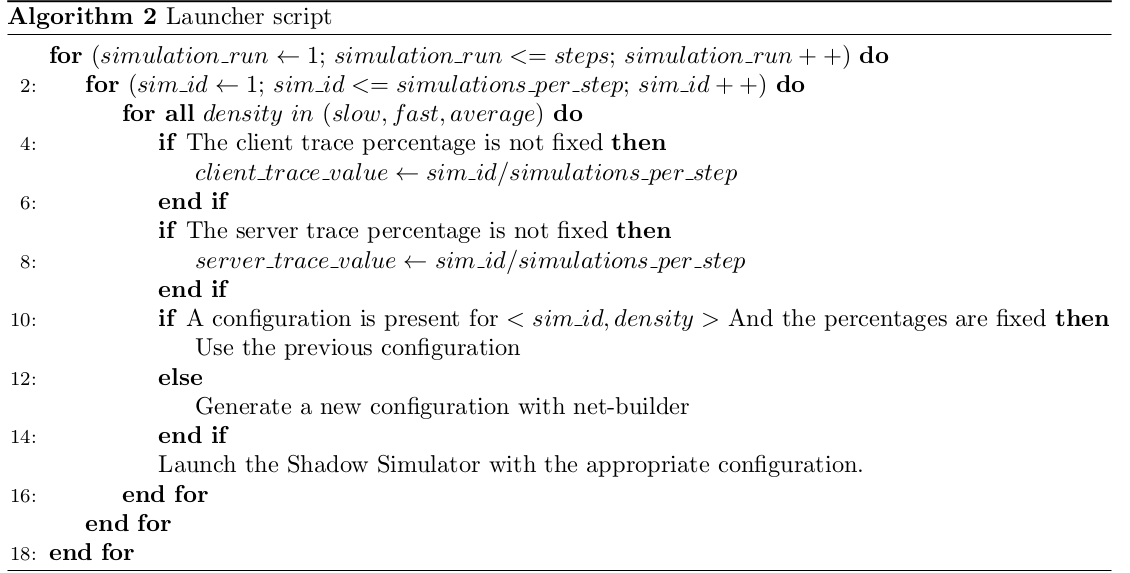
\includegraphics[scale=0.30]{img/algolauncher.png}
		\end{center}				

	\end{frame}

\subsection{Analyzer}
	\begin{frame}{Analyzer}{Log file}
		\begin{center}
			\begin{tabular}{c | c}
			...&$(*)$\\
			c;client10;1420000000&
			s;server7;1421023888\\
			s;server7;1420008031&
			s;server2;1421156205\\
			c;client6;1420005867&
			c;client8;1421160529\\
			s;server9;1420146660&
			s;server3;1421318345\\
			s;server6;1420205384&
			s;server0;1421332488\\
			s;server8;1420252482&
			c;client7;1421487295\\
			c;client0;1420680882&
			c;client4;1421634744\\
			c;client1;1421017740&
			s;server9;1421726485\\
			$(*)$  & ...
			\end{tabular}	
		\end{center}
	\end{frame}

	\begin{frame}{Analyzer}{Scan}
		\begin{itemize}
		 \item For each client connection request $creq$, it looks for candidate
server acceptances
		\item Nested loop ``temporally'' limited between $thr_{MIN}$ (100ms)
$thr_{MAX}$ (6sec)
	\end{itemize}	
	\begin{block}{Time distance}
		Let $\Delta_t(creq, s)$ be the time distance between a $creq$
time-stamp and a server candidate acceptance $s$ time-stamp.
	\end{block}
	
	\end{frame}	
	
	\begin{frame}{Analyzer}{Scan}
		
			\begin{tabular}{ r c | c l }
			&... &$(*)$ &\\
 
			&\textcolor{blue}{\underline{c;client10;1420000000}}&
			s;server7;1421023888&\\
			
			\scriptsize $\Delta_t < thr_{MIN}\to$ &
			\textcolor{red}{s;server7;1420008031}&
			\textcolor{green!90!red!85!blue!85}{s;server2;1421156205}&\\
			
			&c;client6;1420005867&
			c;client8;1421160529&\\
			
			&\textcolor{green!90!red!85!blue!85}{s;server9;1420146660}&
			\textcolor{green!90!red!85!blue!85}	{s;server3;1421318345}&\\
		
			&\textcolor{green!90!red!85!blue!85}{s;server6;1420205384}&
			\textcolor{green!90!red!85!blue!85}{s;server0;1421332488}&\\
		
			&\textcolor{green!90!red!85!blue!85}{s;server8;1420252482}&
			c;client7;1421487295&\\
			
			&c;client0;1420680882&
			c;client4;1421634744&\\
			
			&c;client1;1421017740&
			\textcolor{red}{s;server9;1421726485}&  \scriptsize $\gets$ already
considered\\
			
			&$(*)$  & ... &\\
			\end{tabular}
	\end{frame}

	\begin{frame}{Analyzer}{Matching Probability}
	The likelihood for a server acceptance to be related to a client
request can be related to their time distance.
	\begin{block}{pmatch}
		\begin{equation}
		pmatch(creq, s) = 1 - \frac{\Delta_t(creq, s) - thr_{min}}{thr_{max} - thr_{min}}
		\end{equation}
	\end{block}
	\end{frame}

	\begin{frame}{Analyzer}{Matching Probability}
		\begin{center}
		\begin{minipage}{0.4\textwidth}
		\begin{tabular}{ | c | c |}
			\hline
			candidate &	pmatch\\
			\hline
			server9   &	0.992\\
			server6 &	0.982\\
			server8 &	0.975\\
			server7  &	0.846\\
			server2  &	0.823\\
			server3  &	0.769\\
			server0  &	0.794\\
			... & ... \\
			\hline

		\end{tabular}
		\end{minipage}
		\begin{minipage}{0.4\textwidth}
			The $pmatch$ is higher when the server connection is
closer to $thr_{min}$.
		\end{minipage}
		\end{center}		
	\end{frame}
	
	\begin{frame}{Analyzer}{Time Gap}
		\begin{figure}
			\centering
			
\includegraphics[scale=0.35]{img/gap.png}
		\end{figure}

		\begin{block}{Acceptance Delay Correlation}
		If a server receives a
		connection request from a client after a certain time $\Delta_t$, that
		server will likely receive again another connection from the same client
		after a time that is close to $\Delta_t$ if the Tor communication path is the same as
		before
		\end{block}
	\end{frame}	
	
	\begin{frame}{Analyzer}{Time Gap Average}
As the $pmatch$ is defined as the $\Delta_t$ normalization, let
us define the $gap$ average of a server $s$ marked as candidate for a client $c$ 
		\begin{equation}
		 	gap_{AVG}(c,s) = \frac{\sum\limits^{N(c,s)}_{i=0} 
			| pmatch(creq_{i+1},s) - pmatch(creq_{i},s)|}{N(c,s)}
		\end{equation}
		where $N(c,s)$ is the number of $c$ connection requests that have been likely 
accepted from $s$.

	\end{frame}
		
	\begin{frame}{Analyzer}{Score}
		The $score$ gained by a server $s$ marked as candidate for a
client $c$
		\begin{equation}
			score(c,s) = \frac{\sum\limits^{N(c,s)}_{i=0} pmatch(creq_{i},s)}{gap_{AVG}(c,s) + 1}
		\end{equation}

	\end{frame}

	\begin{frame}{Analyzer}{Best Candidate}
		\begin{center}
			\begin{tabular}{ | c | c || c | c || c | c |  }
				\hline
				\multicolumn{2}{|c||}{client633} &
	\multicolumn{2}{c||}{client637} & \multicolumn{2}{|c|}{client349}\\
				\hline
				\textbf{candidate} 	& \textbf{score} &
\textbf{candidate}  & \textbf{score} & \textbf{candidate} &
\textbf{score} \\
				\hline
				\underline{server8}     & 9.44  & \underline{server3}  &
59.17   & \underline{server0}   & 14.86  \\
				server0     & 7.01  &  server2 & 15.14    & server1   & 13.81\\
				server2 	& 6.88  &  server8 & 13.96    & server5   & 11.94\\
				server5     & 6.83  &  server5 & 8.33     & server2   & 11.20\\
				... 		& ...   &  ... 	   & ...      & ...       & ...\\
				\hline
			\end{tabular}	
		\end{center}
		\begin{block}{Best Candidate}		
			The server candidate with the \textbf{highest score} is the best
			candidate for a certain client.
		\end{block}
	\end{frame}
	\begin{frame}{Analyzer}{Real Data}
		\begin{itemize}
			\item How much are the estimated results close to
the real ones?
			\item Use of real connections logged by the simple-tcp
applications.
			\item Matched accuracy estimation
			\item Matched portion  estimation  
		\end{itemize}
	\end{frame}
		
	\begin{frame}{Analyzer}{Matched Accuracy}
		For each client check if the best candidate is the real server
that accepted its connections and mark it as \textbf{matched}.\\
		\vspace{20pt}
		If so calculate the client accuracy as the distance between the
number of estimated connections $N$ and the number of real connections
$M$:
	\begin{equation}
		 accuracy_c \gets \frac{ MIN(M, N)}{MAX(M, N)}
	\end{equation}
	
	The \emph{matched accuracy} is the average of matched client accuracies.
	
	\end{frame}

	\begin{frame}{Analyzer}{Matched Portion}
		The matched portion indicates how many traced clients 
 			found their real server:
		\begin{equation}
			matched\_portion = \frac{matched_clients}{traced_clients}
		\end{equation}
	\end{frame}
\subsection{Empirical Results}
